\documentclass{article}

\usepackage{graphicx}
\usepackage{tikz}
\usepackage{tikzsymbols}
\usetikzlibrary{calc,patterns,shapes.geometric}
\pagestyle{empty}
\usepackage[margin=0pt]{geometry}
\geometry{papersize={14in,12in}}

\def\centerarc[#1](#2)(#3:#4:#5){\draw[#1] ($(#2)+({#5*cos(#3)},{#5*sin(#3)})$) arc (#3:#4:#5);}

\begin{document}
	\begin{figure}
		\centering
		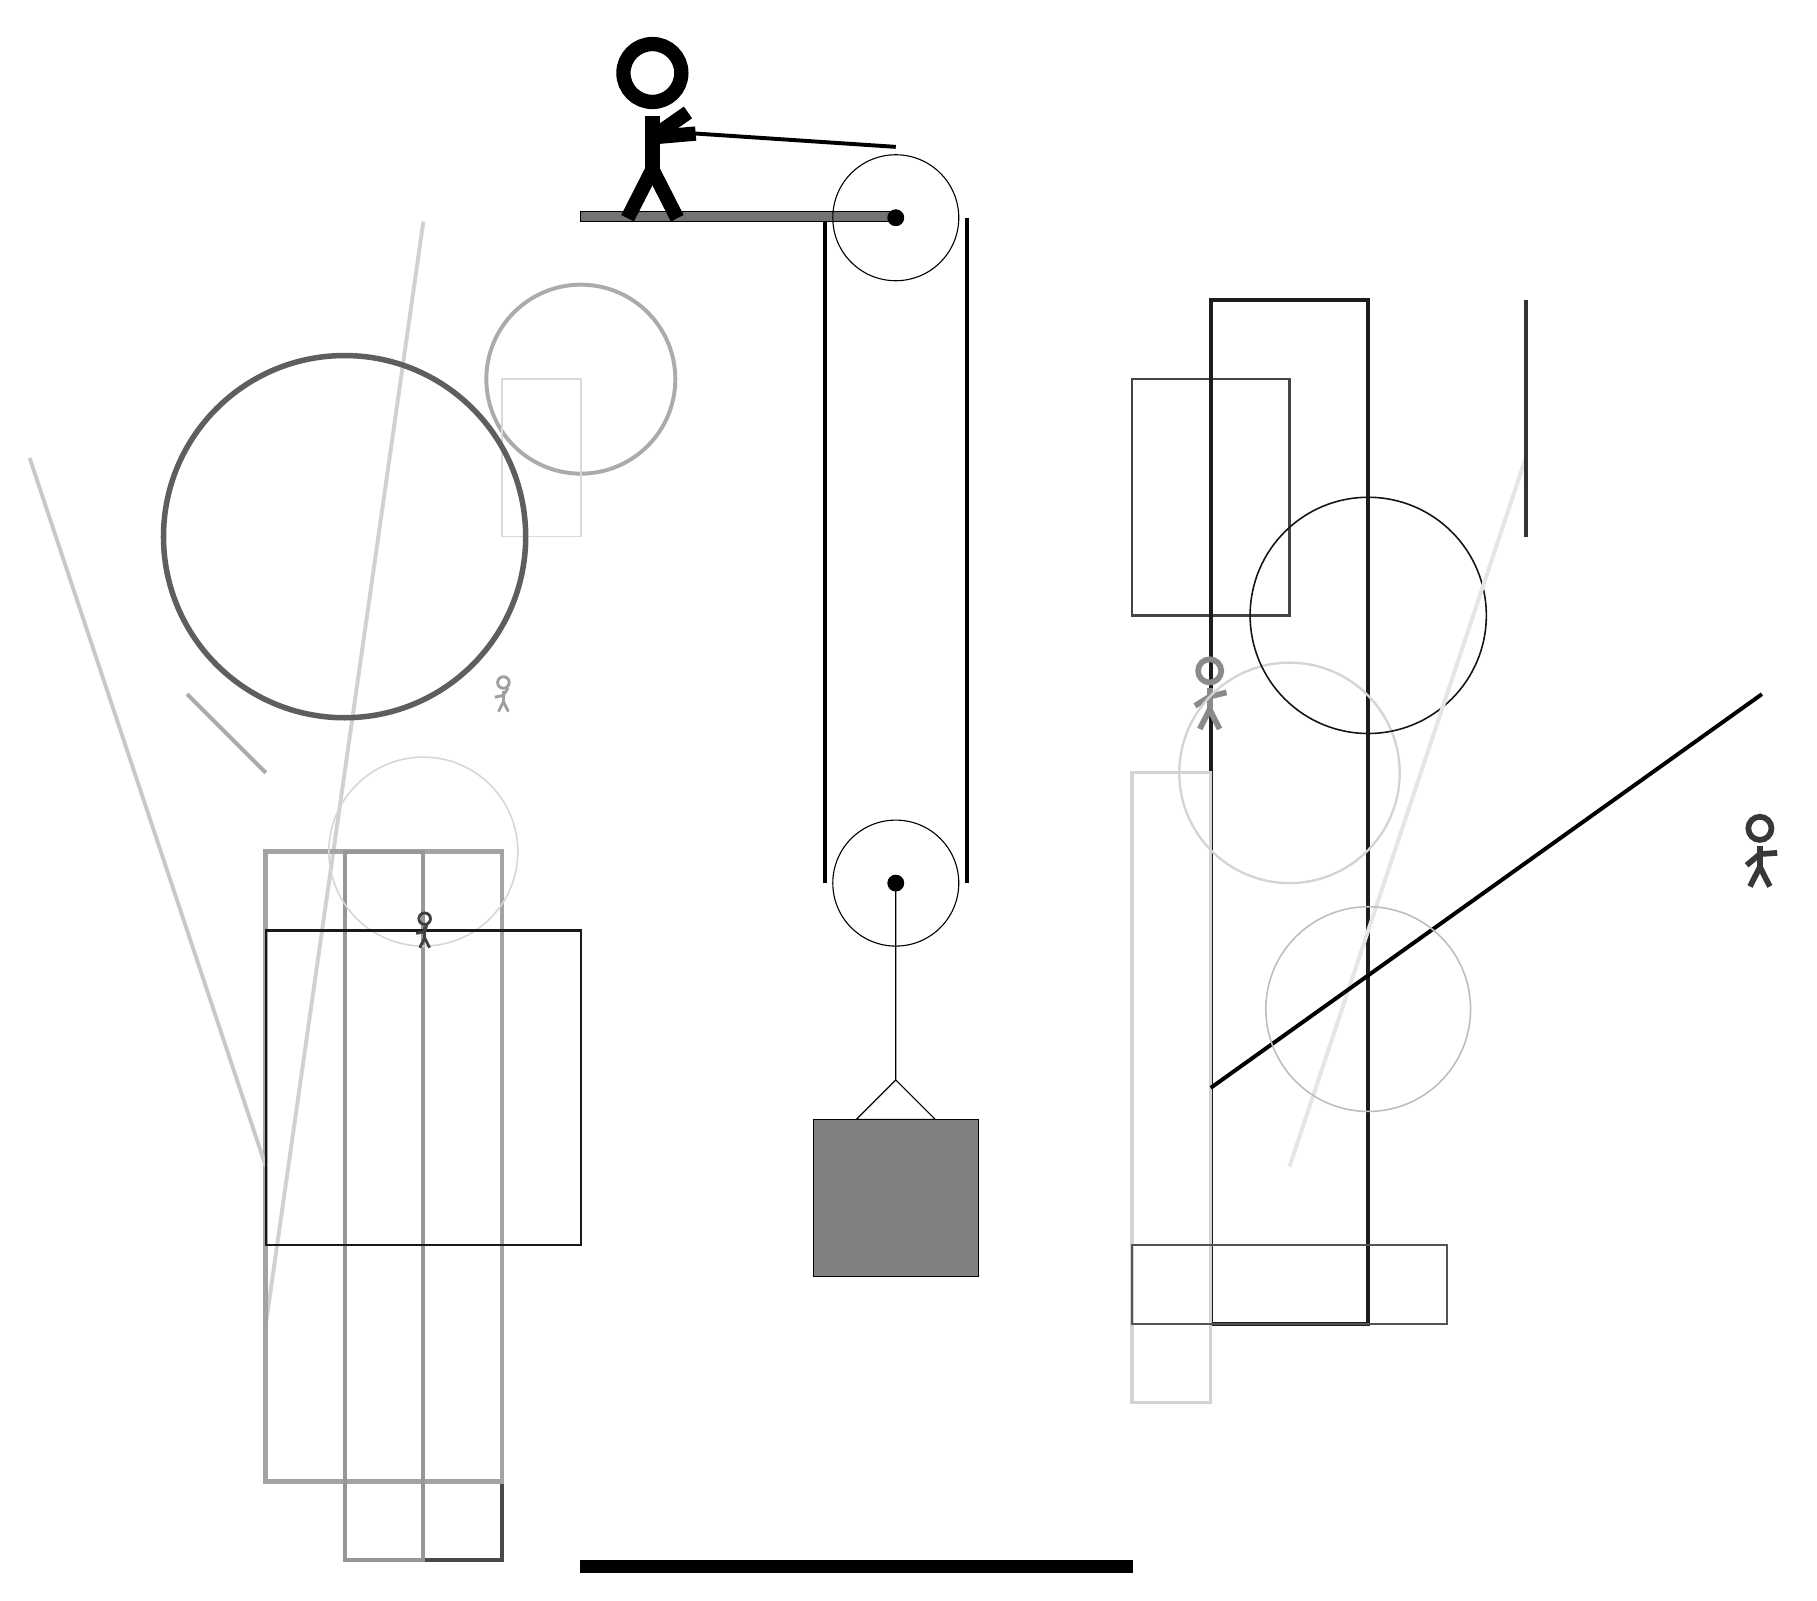
\begin{tikzpicture}
			%%%%% START %%%%%
			
			\draw[fill=black!55] (-2, 14) rectangle (2, 14.125);
			
			\draw (2, 5.6) circle (0.8);
			\draw[fill=black] (2, 5.6) circle (0.1);
			
			\draw [line width=0.4mm, color=black!12](-5, 8) circle (0.0);
			
			\draw [line width=0.5mm, color=black!64](9, 11) circle (0.0);
			\draw[line width=0.3mm, color=black!73] (7, 12) rectangle (5, 9);
			\draw[line width=0.5mm, color=black!18](-4, 14) -- (-6, 0);
			\draw[line width=0.5mm, color=black!71] (-3, -3) rectangle (-5, -2);
			\draw[line width=0.5mm, color=black!89] (6, 13) rectangle (8, 0);
			
			\draw[line width=0.6mm, color=black!36] (-3, -2) rectangle (-6, 6);
			
			\node[line width=0.7mm, color=black!46] at (6, 8) {\Strichmaxerl[4][32][14]};
			\node[line width=0.5mm, color=black!78] at (13, 6) {\Strichmaxerl[4][40][4]};
			\draw[line width=0.5mm, color=black!41] (-4, -3) rectangle (-5, 6);
			
			\draw [line width=0.2mm, color=black!16](-4, 6) circle (1.2);
			\draw[line width=0.5mm, color=black!33](-6, 7) -- (-7, 8);
			\draw [line width=0.5mm, color=black!33](-2, 12) circle (1.2);
			\draw [line width=0.3mm, color=black!17](7, 7) circle (1.4);
			\draw[line width=0.5mm, color=black!21](-6, 2) -- (-9, 11);
			\draw[line width=0.2mm, color=black!15] (-2, 12) rectangle (-3, 10);
			
			\draw [line width=0.7mm, color=black!63](-5, 10) circle (2.3);
			\draw [line width=0.2mm, color=black!92](8, 9) circle (1.5);
			\draw[line width=0.4mm, color=black!17] (6, 7) rectangle (5, -1);
			\draw[line width=0.3mm, color=black!62] (7, 11) rectangle (7, 11);
			\draw[line width=0.3mm, color=black!90] (-2, 5) rectangle (-6, 1);
			\node[line width=0.3mm, color=black!75] at (-4, 5) {\Strichmaxerl[2][12][73]};
			\draw[line width=0.5mm, color=black!10](10, 11) -- (7, 2);
			\node[line width=0.2mm, color=black!38] at (-3, 8) {\Strichmaxerl[2][12][58]};
			\draw[line width=0.5mm, color=black!100](6, 3) -- (13, 8);
			\draw[line width=0.5mm, color=black!80](10, 13) -- (10, 10);
			
			\draw [line width=0.2mm, color=black!26](8, 4) circle (1.3);
			\draw[line width=0.3mm, color=black!67] (5, 1) rectangle (9, 0);
			
			\draw (2, 14.05) circle (0.8);
			\draw[fill=black] (2, 14.05) circle (0.1);
			
			\draw (2, 5.6) -- (2, 3.1) -- (1.5, 2.6) -- (2.5, 2.6) -- (2, 3.1);
			\draw[fill=black!50] (0.95, 2.6) rectangle (3.05, 0.6);
			
			\draw[line width=0.5mm] (1.1, 14) -- (1.1, 5.6);
			\centerarc[line width=0.5mm](2, 5.6)(180:360:0.9);
			\draw[line width=0.5mm](2.9, 5.6) -- (2.9, 14.05);
			\centerarc[line width=0.5mm](2, 14.05)(0:90:0.9);
			\draw[line width=0.5mm](2, 14.95) -- (-1, 15.15);
			
			\node at (-1, 15.15) {\Strichmaxerl[10][-175][35]};
			
			\draw[fill=black] (-2, -3) rectangle (5, -3.15);
			
			%%%%% END %%%%%
		\end{tikzpicture}
	\end{figure}	
\end{document}